As discussed in section \ref{sec:StateOfTheArt}, the TRITIUM consists in a chain of three main elements, plastic scintillating fibers, that produce scintillating photons in response to a tritium electron decay detection, the photosensor, that detects the photons produced in the scintillator and produce an electronic pulse than gives information of the detected photons and the electronic system, which is in charge of processesing and analyzing (first analogically and later digitally) the electrical pulse given by the photosensor. A scheme of a scintillation detector is shown in Figure \ref{fig:ScintillatorDetector}.

\begin{figure}[hbtp]
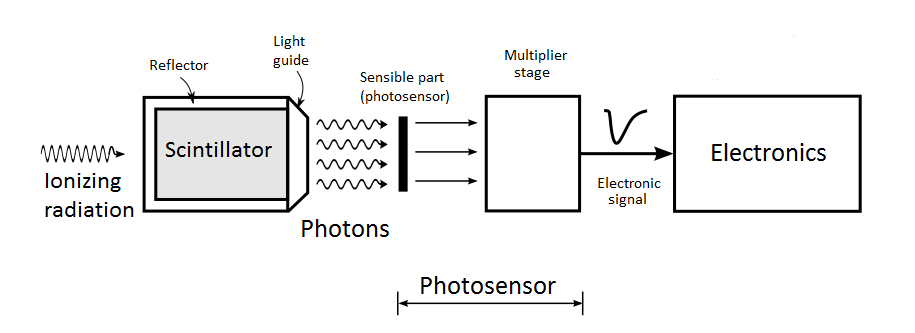
\includegraphics[scale=0.6]{3DesignPrinciples/32Tritium_detector/ScintillatorDetector.png}
\centering
\caption{Scheme of the scintillator detector.\label{fig:ScintillatorDetector}}
\end{figure}
